% Options for packages loaded elsewhere
\PassOptionsToPackage{unicode}{hyperref}
\PassOptionsToPackage{hyphens}{url}
%
\documentclass[
]{book}
\usepackage{lmodern}
\usepackage{amssymb,amsmath}
\usepackage{ifxetex,ifluatex}
\ifnum 0\ifxetex 1\fi\ifluatex 1\fi=0 % if pdftex
  \usepackage[T1]{fontenc}
  \usepackage[utf8]{inputenc}
  \usepackage{textcomp} % provide euro and other symbols
\else % if luatex or xetex
  \usepackage{unicode-math}
  \defaultfontfeatures{Scale=MatchLowercase}
  \defaultfontfeatures[\rmfamily]{Ligatures=TeX,Scale=1}
\fi
% Use upquote if available, for straight quotes in verbatim environments
\IfFileExists{upquote.sty}{\usepackage{upquote}}{}
\IfFileExists{microtype.sty}{% use microtype if available
  \usepackage[]{microtype}
  \UseMicrotypeSet[protrusion]{basicmath} % disable protrusion for tt fonts
}{}
\makeatletter
\@ifundefined{KOMAClassName}{% if non-KOMA class
  \IfFileExists{parskip.sty}{%
    \usepackage{parskip}
  }{% else
    \setlength{\parindent}{0pt}
    \setlength{\parskip}{6pt plus 2pt minus 1pt}}
}{% if KOMA class
  \KOMAoptions{parskip=half}}
\makeatother
\usepackage{xcolor}
\IfFileExists{xurl.sty}{\usepackage{xurl}}{} % add URL line breaks if available
\IfFileExists{bookmark.sty}{\usepackage{bookmark}}{\usepackage{hyperref}}
\hypersetup{
  pdftitle={Analisis Data Sekunder Menggunakan R},
  pdfauthor={Adi Cilik Pierewan},
  hidelinks,
  pdfcreator={LaTeX via pandoc}}
\urlstyle{same} % disable monospaced font for URLs
\usepackage{color}
\usepackage{fancyvrb}
\newcommand{\VerbBar}{|}
\newcommand{\VERB}{\Verb[commandchars=\\\{\}]}
\DefineVerbatimEnvironment{Highlighting}{Verbatim}{commandchars=\\\{\}}
% Add ',fontsize=\small' for more characters per line
\usepackage{framed}
\definecolor{shadecolor}{RGB}{248,248,248}
\newenvironment{Shaded}{\begin{snugshade}}{\end{snugshade}}
\newcommand{\AlertTok}[1]{\textcolor[rgb]{0.94,0.16,0.16}{#1}}
\newcommand{\AnnotationTok}[1]{\textcolor[rgb]{0.56,0.35,0.01}{\textbf{\textit{#1}}}}
\newcommand{\AttributeTok}[1]{\textcolor[rgb]{0.77,0.63,0.00}{#1}}
\newcommand{\BaseNTok}[1]{\textcolor[rgb]{0.00,0.00,0.81}{#1}}
\newcommand{\BuiltInTok}[1]{#1}
\newcommand{\CharTok}[1]{\textcolor[rgb]{0.31,0.60,0.02}{#1}}
\newcommand{\CommentTok}[1]{\textcolor[rgb]{0.56,0.35,0.01}{\textit{#1}}}
\newcommand{\CommentVarTok}[1]{\textcolor[rgb]{0.56,0.35,0.01}{\textbf{\textit{#1}}}}
\newcommand{\ConstantTok}[1]{\textcolor[rgb]{0.00,0.00,0.00}{#1}}
\newcommand{\ControlFlowTok}[1]{\textcolor[rgb]{0.13,0.29,0.53}{\textbf{#1}}}
\newcommand{\DataTypeTok}[1]{\textcolor[rgb]{0.13,0.29,0.53}{#1}}
\newcommand{\DecValTok}[1]{\textcolor[rgb]{0.00,0.00,0.81}{#1}}
\newcommand{\DocumentationTok}[1]{\textcolor[rgb]{0.56,0.35,0.01}{\textbf{\textit{#1}}}}
\newcommand{\ErrorTok}[1]{\textcolor[rgb]{0.64,0.00,0.00}{\textbf{#1}}}
\newcommand{\ExtensionTok}[1]{#1}
\newcommand{\FloatTok}[1]{\textcolor[rgb]{0.00,0.00,0.81}{#1}}
\newcommand{\FunctionTok}[1]{\textcolor[rgb]{0.00,0.00,0.00}{#1}}
\newcommand{\ImportTok}[1]{#1}
\newcommand{\InformationTok}[1]{\textcolor[rgb]{0.56,0.35,0.01}{\textbf{\textit{#1}}}}
\newcommand{\KeywordTok}[1]{\textcolor[rgb]{0.13,0.29,0.53}{\textbf{#1}}}
\newcommand{\NormalTok}[1]{#1}
\newcommand{\OperatorTok}[1]{\textcolor[rgb]{0.81,0.36,0.00}{\textbf{#1}}}
\newcommand{\OtherTok}[1]{\textcolor[rgb]{0.56,0.35,0.01}{#1}}
\newcommand{\PreprocessorTok}[1]{\textcolor[rgb]{0.56,0.35,0.01}{\textit{#1}}}
\newcommand{\RegionMarkerTok}[1]{#1}
\newcommand{\SpecialCharTok}[1]{\textcolor[rgb]{0.00,0.00,0.00}{#1}}
\newcommand{\SpecialStringTok}[1]{\textcolor[rgb]{0.31,0.60,0.02}{#1}}
\newcommand{\StringTok}[1]{\textcolor[rgb]{0.31,0.60,0.02}{#1}}
\newcommand{\VariableTok}[1]{\textcolor[rgb]{0.00,0.00,0.00}{#1}}
\newcommand{\VerbatimStringTok}[1]{\textcolor[rgb]{0.31,0.60,0.02}{#1}}
\newcommand{\WarningTok}[1]{\textcolor[rgb]{0.56,0.35,0.01}{\textbf{\textit{#1}}}}
\usepackage{longtable,booktabs}
% Correct order of tables after \paragraph or \subparagraph
\usepackage{etoolbox}
\makeatletter
\patchcmd\longtable{\par}{\if@noskipsec\mbox{}\fi\par}{}{}
\makeatother
% Allow footnotes in longtable head/foot
\IfFileExists{footnotehyper.sty}{\usepackage{footnotehyper}}{\usepackage{footnote}}
\makesavenoteenv{longtable}
\usepackage{graphicx}
\makeatletter
\def\maxwidth{\ifdim\Gin@nat@width>\linewidth\linewidth\else\Gin@nat@width\fi}
\def\maxheight{\ifdim\Gin@nat@height>\textheight\textheight\else\Gin@nat@height\fi}
\makeatother
% Scale images if necessary, so that they will not overflow the page
% margins by default, and it is still possible to overwrite the defaults
% using explicit options in \includegraphics[width, height, ...]{}
\setkeys{Gin}{width=\maxwidth,height=\maxheight,keepaspectratio}
% Set default figure placement to htbp
\makeatletter
\def\fps@figure{htbp}
\makeatother
\setlength{\emergencystretch}{3em} % prevent overfull lines
\providecommand{\tightlist}{%
  \setlength{\itemsep}{0pt}\setlength{\parskip}{0pt}}
\setcounter{secnumdepth}{5}
\usepackage{booktabs}
\usepackage[]{natbib}
\bibliographystyle{apalike}

\title{Analisis Data Sekunder Menggunakan R}
\author{Adi Cilik Pierewan}
\date{2020-05-05}

\begin{document}
\maketitle

{
\setcounter{tocdepth}{1}
\tableofcontents
}
\hypertarget{pengantar}{%
\chapter{Pengantar}\label{pengantar}}

Buku ini akan memberi panduan bagaimana menggunakan data sekunder untuk penelitian dan implementasinya dalam pemrograman R.

The \textbf{bookdown} package can be installed from CRAN or Github:

\begin{Shaded}
\begin{Highlighting}[]
\KeywordTok{install.packages}\NormalTok{(}\StringTok{"bookdown"}\NormalTok{)}
\CommentTok{\# or the development version}
\CommentTok{\# devtools::install\_github("rstudio/bookdown")}
\end{Highlighting}
\end{Shaded}

Remember each Rmd file contains one and only one chapter, and a chapter is defined by the first-level heading \texttt{\#}.

To compile this example to PDF, you need XeLaTeX. You are recommended to install TinyTeX (which includes XeLaTeX): \url{https://yihui.org/tinytex/}.

\hypertarget{lanskap-penelitian-data-sekunder}{%
\chapter{Lanskap penelitian data sekunder}\label{lanskap-penelitian-data-sekunder}}

\hypertarget{pengantar-1}{%
\section{Pengantar}\label{pengantar-1}}

Ada dua kondisi yang memotivasi buku ini: revolusi komputer dan ketersediaan data. Revolusi komputer memungkinkan penliti untuk melakukan komputasi secara modern dan pemodelan pada data yang menyediakan wawasan untuk pengembangan ilmu dan pembuatan kebijakan. Kedua, ketersediaan data merupakan peluang emas bagi para peneliti dan ilmuwan untuk melakukan kajian yang intensif mengenai isu sosial dan yang terkait. Buku ini dibuat untuk menambah referensi mengenai analisis data sekunder. Buku ini merupakan buku teori dan panduan mengenai analisis data sekunder yang bertujuan untuk memberi wawasan dan keterampilan untuk melakukan penelitian menggunakan data sekunder. Buku ini akan berisi tentang definisi, teori dan praktik untuk melakukan penelitian data sekunder.

Masalah sosial terjadi di penjuru dunia. Dunia saat ini banyak menyediakan data. Dua fakta tersebut merupakan fakta yang tidak terelakkan dan terkait satu dan yang lain. Masalah sosial dapat direkam melalui data dan data dapat membantu untuk menjadi solusi pemecahan masalah sosial. Hal inilah hyang menjadi motivasi awal penulisan buku ini.

British Academy (2012) menyatakan adanya krisis literasi data dan statistika di kalangan ilmu sosial dan humaniora. Padahal kenyataan yang ada adalah adanya fenomena big data dan fenomena masyarakat digital hyang memproduksi data, atau dalam bahasa Ritzer (2010) disebut masyarakat prosumer, produsen sekaligus konsumer data.

Gambaran yang diberikan oleh British Academy hampir sama apa yang dialami apa yang terjadi di Indonesia, dimana minat dan keterampilan dalam keterampilan kuantitatif di kalangan ilmuwan sosial di Indonesia. Tradisi kuantitatif yang kuat ada dalam bidang psikologi dan ekonomi. Namun demikian, fakta mengenai big data dan perubahan sosial yang sangat cepat merupakan salah satu motivasi yang kuat untuk mendalami metode kuantitatif dalam ilmu sosial.

Penggunaan data sekunder pada penelitian saat ini, tidak terlepas dari sebuah gerkana intelektual yang disebut dengan artimetika politis, yaitu sebuah penggunaan angka untuk mempengaruhi kebijakan pemerintah. Penggunaan angka tersebut dapat secara akurat membantu pemerintah untuk mengambil keputusan yang akan diambil untuk kesejahteraan masyarakat (Smith, 2008).

\hypertarget{mengapa-data-sekunder}{%
\chapter{Mengapa Data Sekunder}\label{mengapa-data-sekunder}}

\hypertarget{keuntungan-data-sekunder}{%
\section{Keuntungan data sekunder}\label{keuntungan-data-sekunder}}

Beberapa keuntungan yang dapat diperoleh ketika kita menggunakan data sekunder antara lain: murah dan efisien. Penelitian yang dilakukan dapat segera diketahui hasilnya tanpa melakukan penelitian di lapangan. Dengan demikian, peneliti dapat menulis hasil penelitian dan seghera diterbitkan pada jurnal bereputasi.

Keuntungan yang paling nampak adalah ekonomi. Data sekunder sudah dikumpulkan oleh orang lain atau pihak lain, sehingga tidak diperlukan biaya yang dibutuhkan untuk mengumpulkan data. Selain itu, waktu yang dibutuhkan untuk mengumpulkan data juga dapat diminimalisasi.

Keuntungan kedua adalah luasnya jangkauan data yang disediakan oleh data sekunder. Keluasan ini dapat dilihat dari jumlah pertanyaan yang banyak dan responden yang banyak., sehingga keterwakilan untuk populasi menjadi lebih meyakinkan.

Keuntungan ketiga, proses pengumpulan dalam data sekunder dilakukan oleh orang-orang yang ahli dalam bidang survey dan juga dalam isu substantif sehingga kuesioner yang ada dapat digunakan untuk melakukan analisis dengan pemodelan yang kompleks.

Keuntungan keempat, data sekunder dapat digunakan untuk bahan mengajar di tingkat sarjana dan pascasarjana karena data yang tersedia sudah ada dan tidak memerlukan sumber daya yang mahal. Sautter (2014) menunjukkkan bagaimana data sekunder dapat digunakan secara efektif untuk membantu pengajaran Metode Penelitian dan Statistika Sosial pada mata kuliah ilmu sosial. Sebelumnya, Howery (2006) sudah melakukan inisiasi untuk mengintegrasikan data sekunder pada pembelajaran substantif dalam bidang sosiologi.

\#\#Kelemahan data sekunder

Kerugian ketika menggunakan data sekunder antara lain: tidak sesuai dengan pertanyaan penelitian dan jangkauan topik penelitian terlalu luas.

Kelemahan yang utama dari penelitian data sekunder adalah tidak bisa menjawab pertanyaan penelitian yang spesifik karena survey yang didesain mungkin tidak secara spesifik terkait dengan pertanyaan penelitian yang diajukan.

Kelemahan kedua yaitu ketidakterlibatan penelitian pada proses pengumpulan data mengakibatkan peneliti tidak memiliki pemahaman yang baik dan komprehensif terhadap data yang ada.

\hypertarget{penerapan-data-sekunder-pada-ilmu-sosial}{%
\section{Penerapan data sekunder pada ilmu sosial}\label{penerapan-data-sekunder-pada-ilmu-sosial}}

Sosiologi

Data sekunder dalam bidang studi sosiologi dapat dijumpai pada data understanding society (), European Values Study (). Data yang ada dalam kajian ini termasuuk data yang terkait dengan sosiologi kesehatan atau epidemiologi sosial. Robert Sampson, Harvard University yang melakukan penelitian dengan data sekudner yang emngambil wilayah kota Chicago, dengan proyek penelitian besar yang dinamai Neighborhood Effects. Dalam penliyian ini Sampson berhasil menyimpulkan tentang bagaimana mekanisme spasial terjadi dan bagaimana ikmuwan sosial dapat menjawab pertanyaan penelitian menegani fenomena tersebut.

Ekonomi

Data sekunder dalam bidang ekonomi dapat dilihat pada data IFLS, dimana banyak dijumpai variabel yang terkait dengan kajian ekonomi termasuk pemngambilan keputusan, tingkat kesejahteraan ekonomi masyarakat. Angus Deaton, peraih Nobel Ekonomi 2016 merupakan pengguna data sekunder. Paper yang ditulis kebanyakan adalah data sekunder yang didekati dengan pemodelan yang tepat untuk menjawab pertanyaan penting dalam bidang ekonomi. Para ekonom studi pembangunan memiliki minat yang tinggi terhadap data sekunder, misalnya di Indonesia mereka banhyak menggunakan data SUSENAS yang diselenggarakan oleh BPS.

Geografi

Data sekunder yang mencakup data geografi memasukkan unsur spasial atau data yang terkait dengan kondisi geografis dan lingkungan yang ada dalam masyarakat. Contoh data ini dapat dilihat dalam PHDCN hyang mengkaji kesejahteraan sosial masyarakat kota Chicago. Geograf di UK dan US banyak melakukan penlitian menggunakan data sekunder. Sebagai contoh JAmes Cheshire mencpba memetakan fenomena sosial di London dan UK, menggunakan data sekunder atau bahkan dengan teknologi data besar.

Kajian demografi termasuk kajian geografi dan merupakan salah satu bidang dalam ilmu sosial yang menyediakan data yang banyak di tingkat nasional dan internasional. Data ini biasanya disediakan oleh badan resmi statistika di masing-masing negara. Kajian interdisiplin yang menggunakan perspektif spasial ,banyak menggunakan informasi geografis untuk menjelaskan bagaimana peran lokasi dapat menjelaskan fenomena sosial. Data-data spasial, saat ini banyak ditemukan pada banyak survey dan juga badan resmi statistika di masing-masing negara. Sebagai contoh Office National for Statistics (ONS) \url{https://www.ons.gov.uk/} yang menyediakan informasi spasial yang detail hingga di tingkat tetangga atau disebut dengan LSOA (Lower Super Output Area). Informasi ini sangat bermanfaat untuk menjelaskan bagaimana lokasi rumah tertentu dapat memrediksikan kondisi sosial yang dialami orang tersebut.

Psikologi

Data sekunder dalam bidang psikologi dimasukkan dalam survey antara lain IFLS yang memasukkan tingkat depresi dan kondisi emosi individu. Psikologi merupakan bidang ilmu yang paling terakhir dalam menggunakan data sekunder. Hal ini wajar karena tradisi penelitian dalam psikologi kebanyakan menggunakan data primer yang sesuai dengan tema atau topik yang dipilih peneliti. Nsmun demikian, lima tahun terakhir ini ilmuwan psikologi mulai banyak menggunakan data sekunder, mengingat mulai banyaknya data yang tersedia yang menyediakan pertanyaan psikologis pada survey tingkat nasional maupun internasional, misalnya mengenai kesejahteraan subjektif dan emosi warga.

Ilmu politik

Data sekunder dalam bidang politik dapat dijumpai pada EVS dan ESS yang mencakup bagaimana nilai sebuah masyarakat dan bagaimana sikap politik dan partisipasi politik warga. Pada laman ICPSR University of Michigan, kita dapat menjumpai banyak survey yang terkait dengan kajian politik, terutama bagaimana respon dan sikap warga pada kondisi politik pada negara mereka.

Ilmu politik juga banyak mengoptimalkan data yang berasal dari polling pada saat pemilihan umum atau pemilihan kepala daerah. Dalam survey sosial, ilmu politik memberi kontribusi yang besar terutama dalam melihat bagaimana masyarakat memiliki pandangan politik tertentu.

Pendidikan

Data sekunder dalam bidang pendidikan yang sangat populer adalah PISA yang dikeluarkan oleh OECD dan TIMSS. Dua survey ini sering dijadikan barometer untuk kemajuan sebuah negara dibandingkan negara lain di seluruh dunia. Selain itu, soal-soal yang digunakan di PISA atau TIMSS banyak digunakan untuk standar ujian pada siswa sekolah di sejumlah negara di dunia. PISA dapat diunduh secara gratis melalui link berikut ini \url{https://www.oecd.org/pisa/pisaproducts/}, sedangkan TIMSS dapat diunduh melalui link berikut \url{http://timssandpirls.bc.edu/}.

Kebijakan Publik

Data sekunder dalam kebijakan publik sangat populer dilakukan. Kajian kebijakan publik merupakan salah bidang yang paling diuntungkan penggunaan data sekunder dalam penelitian, karena jangkauan penelitian dengan data sekunder ini bersifat luas dan generalisasinya dapat digunakan untuk membantu pembuatan kebijakan publik.

Bidang kebijakan publik merupakan salah satu bidang yang paling banyak memperoleh keuntungan penggunaan data sekunder untuk pembuatan kebijakan yang efektif. Dalam kajian pengambilan kebijakan, kajian ini sering disebut dengan pembuatan kebijakan berbasis data atau bukti yang akurat atu evidence-based decision making. Sebuah stretegi yang bersandara dengan data dan kejadian, yang pada tahap selanjutnya dibuat menjadi sebuah kebijakan yang dapat diterima masyarakat dan pihak terkait.

\hypertarget{proses-dan-identifikasi-data-sekunder}{%
\chapter{Proses dan Identifikasi Data Sekunder}\label{proses-dan-identifikasi-data-sekunder}}

\#\#Proses

Proses melakukan penelitian data sekunder dapat dilakukan seperti penelitian pada umumnya, namun salah satu proses yang dapat diubah adalah tentang bagaimana mengidemtifikasi data yang sesuai dengan penelitian kita. Pada penelitian data sekunder, kita dapat melakukan penelitian dengan dimulai mencari data yang ada dalam riset tersebut, atau bahkan mencari jurnal yang menggunakan data tersebut. Kita dapat menemukan penelitian, sebagai contoh, pada laman web berikut ini: \url{http://www.rand.org/labor/FLS/IFLS/papers.html}. Laman tersebut memberikan contoh tentang bagaimana penelitian data sekunder dilakukan dengan menggunakan data IFLS. Dengan mencermati penelitian tersebut, kita dapat mempelajari bagaimana data sekunder ditemukan, dianalisis dan ditulis sebagai makalah ilmiah yang diterbitkan dalam jurnal bereputasi.

Proses penelitian dapat dilakukan dengan proses berikut ini Boslaugh (2007) :

\begin{enumerate}
\def\labelenumi{\arabic{enumi}.}
\item
  Mendefinisikan pertanyaan penelitian. Seperti proses penelitian standar, pertanyaan penelitian data sekunder perlu dimulai dengan pertanyaan penelitian yang jelas.
\item
  Menentukan target responden. Target responden perlu dijelaskan sejak awal.
\item
  Menentukan variabel lain yang akan dimasukkan dalam analisis.
\item
  Menentukan jenis data yang paling cocok dengan pertanyaan penelitian.
\item
  Membuat daftar data yang mencantumkan informasi yang terkait dengan pertanyaan penelitian.
\item
  Uji variabel yang kita gunakan.
\end{enumerate}

Penulis ingin berbagi pengalaman melakukan penelitian sekunder mulai dari awal sampai pada akhir pengiriman naskah publikasi.

Menentukan topik penelitian

Topik penelitian harus ditentukan sejak awal agar penelitian kita lebih sejalan dengan apa yang kita inginkan. Menentukan topik merupakan salah satu tahapan paling menantang bagi ilmuwan sosial terutama bagi pemula, karena banyak sekali topik yang menarik namun demikian peneliti pemula merasakan kesulitan untuk melakukan fokus pada satu topik secara intens.

Melakukan pencarian pada jurnal yang terkait

Langkah selanjtnya adalah mencari jurnal yang terkait dengan topik kita. Pencarian jurnal sekarang dapat dilakukan dengan mudah. Banyak website yang bisa menyediakan jurnal secara gratis yang langsung disediakan oleh penulisnya, misalnya pada laman ini: \url{https://www.researchgate.net/home}. Pada laman ini kita bisa melihat paper yang ditulis oleh penulis yang memiliki minat sama dengan kita. Pendek kata, laman ini merupakan media jaringan sosial akademik.

Membaca dengan seksama jurnal yang terpilih

Langkah selanjutnya adalah membaca artikel dengan seksama dan detail, sehingga kita bisa mengetahui alur logika yang digunakan oleh penulis tersebut. Proses membaca ini dilakukan dengan mengkritisi paper yang sedang kita baca dengan cara menemukan kelemahan argumen yang diberikan dalam paper tersebut.

Melakukan replikasi penelitian

Replikasi penelitian dilakukan untuk mengetahui lebih dalam bagaiaman penelitian terdahulu dilakukan dan pada waktu yang sama memberikan rasa pencapaian dari peneliti yang bahwa yang bersangkutan bisa menyelesaikan penelitian serupa. Penulis melakukan replikasi penelitian yang dilakukan oleh Paxton (2007) mengenai association membership and trust dan saat itu penulis meminta data secara langsung dari Paxton, dan Paxton juga memberi data tersebut. Proses selanjutnya adalah melakukan analisis untuk data yang tersedia dan hasilnya hampir sama apa yang dilakukan Paxton.

Mencari data set yang relevan

Data set yang relevan sangat perlu dilakukan sesuai dengan topik kita dengan membaca kuesioner dan mencermati codebook yang ada, sehingga peneliti dapat mengidentifikasi masing-masing item atau pertanyaan yang relevan. Saat itu, penulis mencermati dua data set yaitu European Social Survey dan European Values Study. Kedua data set tersebut menyediakan informasi mengani nilai dan perubahan sosial yang terjadi di Eropa. Setelah mencermati kedua dat set tersebut, akhirnya dipilih salah satu dat set yaitu EVS, karena yang menyediakan pertanyaan sesuai dengan topik yang sudah dipilih.

Melakukan penelitian dengan topik terpilih

Setelah menemukan topik, langkah selanjutnya adalah melakukan penelitian formal dengan data yang sudah kita ambil. Penelitian ini dilakukan seperti penelitian dengan data primer yaitu dengan menentukan pertanyaan penelitian yang akan dijawab dalam penelitian dan melakukan pengujian menggunakan analisis data yang relevan untuk menjawab pertanyaan penelitian.

Mencari jurnal yang terkait dengan strategi penelitian.

Mencari jurnal merupakan salah satu langkah paling menentukan dalam penelitian data sekunder. Fungsi pemilihan jurnal ini adalah: memberi tuntunan pada proses penelitian yang akan dilakukan.

Melakukan analisis data

Memilih perangkat lunak

Proses pemilihan lunak sangat disesuaikan dengan kebutuhan penelitian dan penjelasan lebih detail ada pada Bab 5. Pemilihan ini didasarkan pada ketersediaan sumber daya yang ada, termasuk dana yang tersedia. Perangkat lunak saat tersedia secara luas dan mudah untuk diperoleh, namun diperlukan waktu yang cukup untuk menguasai perangkat yang tersedia tersebut.

Mencari jurnal yang relevan dengan teknik analisis yang sudah dipilih

Pada saat data set dan jurnal teoretis sudah ditemukan, maka selanjutnya mencari jurnal yang menggunakan teknik analisis hyang sesuai dengan penelitian kita. Saat itu, peneliti mencari jurnal yang menggunakan penelitian multilevel model untuk menjawab pertanyaan tentang apakah variasi di level yang lebih tinggi dapat menjelaskan fenomena pada level-1.

Mempublikasikan pada jurnal relevan

Saat yang paling menggembirakan adalah ketika penelitian kita sudah jadi dan siap untuk dipublikasikan pada jurnal yang relevan. Pada saat itu, saya memilih dua jurnal untuk dipublikasikan yaitu Social Indicators Reserach dan Jornal of Happiness Studies. Artikel saya ditolak di JOHS, akhirnya saya kirim lagi ke SIR. Akhirnya SIR menerima artikel saya dan siap dipublikasikan. Menerima surat penerimaan di jurnal yang kita merupakan pengalaman yang yang tidak terlupakan, karena saat itulah saya merasa karir akademik saya dimulai secara internasional.

\#\#Sumber data sekunder

Data sekunder dapat diperoleh baik dari sumber di Indonesia dan luar negeri. Di Indonesia kita dapat menemukan data sekunder dari BPS dan survey yang dilakukan oleh lembaga survey atau lembaga penelitian terkemuka di Indonesia. Salah satu survey yang menyediakan banyak pertanyaan dan wahana untuk melakukan analisis data sekunder adalah Survey Aspek Kehidupan Rumah Tangga Indonesia (SAKERTI) atau dikenal secara internasional sebagai Indonesia Family Life Survey (IFLS) \url{http://www.rand.org/labor/FLS/IFLS.html}.

\#\#\#Sumber data internasional

Sumber data internasional bisa diperoleh dari PBB, Bank Dunia, lembaga survey internasional , seperti Gallup Internasional, World Values Survey. Di UK, dapat penyedia layanan data dapat ditemukan pada web ini: UKDS \url{https://www.ukdataservice.ac.uk/}. Di Jerman, layanan data di tingkat Eropa dan dunia dapat ditemukan pada link berikut: GESIS \url{http://www.gesis.org/en/services/}. Sedangan di Amerika kita dapat menemukannya di ICPSR University of Michigan \url{http://www.icpsr.umich.edu/icpsrweb/}. Ketiga pengelola data internasional tersebut, dapat memberikan layanan data, dan analisis data yang kompleks untuk kepentingan pembuatan kebijakan publik. Bahkan pusat peneydia data tersebut membrikan kesempatan untuk melakukan penelitian di institusi mereka dan bisa mengakses data yang dimiliki dan perangkat lunak yang dibutuhkan untuk menganalisis.

\#\#\#Sumber data regional

Contoh sumber data regional EVS, EuroBarometer, AsiaBarometer. Data tersebut tersimpan di arsip data antara lain pada link berikut ini. EVS diselenggarakan oleh European Values Foundation yang menyediakan pelayanan survey untuk mengetahui bagaimana nilai dan perubahan sosial dialami oleh penduduk Eropa dan terjadi di Eropa. Data ini dapat ditemukan di link berikut: \url{http://www.europeanvaluesstudy.eu/page/surveys.html}. Sedangkan untuk data Eropa yang lain dapat ditemukan pada European Social Survey, \url{http://www.europeansocialsurvey.org/data/round-index.html}. Hampir sama dengan EVS, ESS mengumpulkan data mengenai perubahan sosial yang terjadi di Eropa. Survey ini sudah berlangsung sejak 2002 dan diselenggarakan setiap dua tahun, dan untuk wave terakhir dilakukan pada tanggal 2014. Surevy ini juga menyediakan data yang terintegrasi, yang sudah digabungkan antara data di tingkat individu dan data kontekstual yang memungkinkan untuk melakukan analisis multilevel dan pemodelan kompleks dalam ilmu sosial. Di tingkat Asia, tersedia data Asibarometer \url{http://www.asianbarometer.org/} mengkaji nilai politik dan demokrasi diantara warga Asia.

\#\#\#Sumber data nasional

Sumber data di tingkat nasional yang dianalisis antara lain sumber data yang berasal dari pemerintah dan survey di tingkat nasional. Di UK data untuk data sekunder tersimpan di ESDS atau UKDA \url{http://www.data-archive.ac.uk/}. Di US data sekunder tersimpan ICPSR University of Michigan \url{http://www.icpsr.umich.edu/icpsrweb/}. Sumber data tersebut tidak hanya menyediakan data yang terkait dengan data di tingkat nasional, namun juga menyediakan data internasional. UKDA, sebagai contoh, menyediakan data yang memuat survey di Jepang, yang termasuk survey tingkat nasional. Selain itu UKDA menyediakan perangkat analisis online yang dapat digunakan secara langsung oleh peneliti walaupun untuk analisis deskriptif yang sederhana. ICPSR juga menyediakan fasilitas serupa, dan dapat digunakan oleh peneliti sosial sekaligus juga menyediakan perangkat untuk pembelajaran yang baik untuk mengenalkan data yang terkait dengan isu kependudukan dan perubahan sosial. Perangkat pembelajaran yang menggunakan data sekunder dapat ditemukan dalam laman ini \url{https://www.icpsr.umich.edu/icpsrweb/content/instructors/teacher-resources.html}. Laman tersebut dapat membantu mahasiswa lebih paham pada data dan penggunaannya untuk pembelajaran ilmu sosial. Dengan menggunakan pendekatan ini, dosen dan mahasiswa dapat lebih memahami tidak secara teoretis namun juga secara empiris mengenai fenomena sosial yang ada baik secara nasional maupun secara internasional.

Sumber data di tingkat nasional dapat dijumpai pada survey terkenal di beberapa negara maju, antara lain di Amerika mereka mengadakan General Social Survey (GSS), di Inggris dikenal dengan Understanding Society, dan di Jerman mereka menyelenggarakan German Social Economic Panel (GSOEP). Semua survey tersebut memberikan data yang relatif lengkap yang mencakup isu sosial, ekonomi dan politik yang krusial dan mencakup pemahaman antar waktu.

\hypertarget{memahami-codebook}{%
\chapter{Memahami codebook}\label{memahami-codebook}}

\hypertarget{pertanyaan-penelitian}{%
\chapter{Pertanyaan Penelitian}\label{pertanyaan-penelitian}}

\hypertarget{memahami-r}{%
\chapter{Memahami R}\label{memahami-r}}

\hypertarget{mengapa-r}{%
\section{Mengapa R}\label{mengapa-r}}

Salah satu keunggulan menggunakan R adalah menyediakan fitur yang lengkap untuk analisis data dan visualisasi data, sedangkan dapat diperoleh secara gratis.

\hypertarget{manajemen-data}{%
\subsection{Manajemen Data}\label{manajemen-data}}

Manajemen data merupakan proses paling emnantang dalam analisis data pada umumnya dan analisis data sekunder pada umumnya. Salah satu perngkat lunak yang bisa digunakan untuk melakukan manajemen data adalah STATA, biasanya digunakan oleh ahli ekonometri dan kesehatan masyarakat. Namun demikian, STATA merupakan perangkat lunak berbayar, sehingga penulis mnyarakan untuk menggunakan R dengan paket dplyr yang mempunyai kemampuan yang baik untuk melakukan manajemen data denngan baik dan dapat dilakukan dengan relatif mudah.

Manajemen data merupakan proses paling menentukan dalam proses analisis data. Jika penelit tidak melakukan manjemen data dengan baik, maka kemungkinan yang akan terjadi adalah kesalahan dalam melakukan analisis data atau estimasi. Misalnya, jika satu variabel seharusnya dihitung secara terbalik, namun tidak dibalik oleh peneliti, maka hasilnya dapat menyesatkan.

Manajemen data dengan R akan lebih mudah jika menggunanakan paket dplyr.

\begin{verbatim}
knitr::include_graphics(rep("rmda.png"))
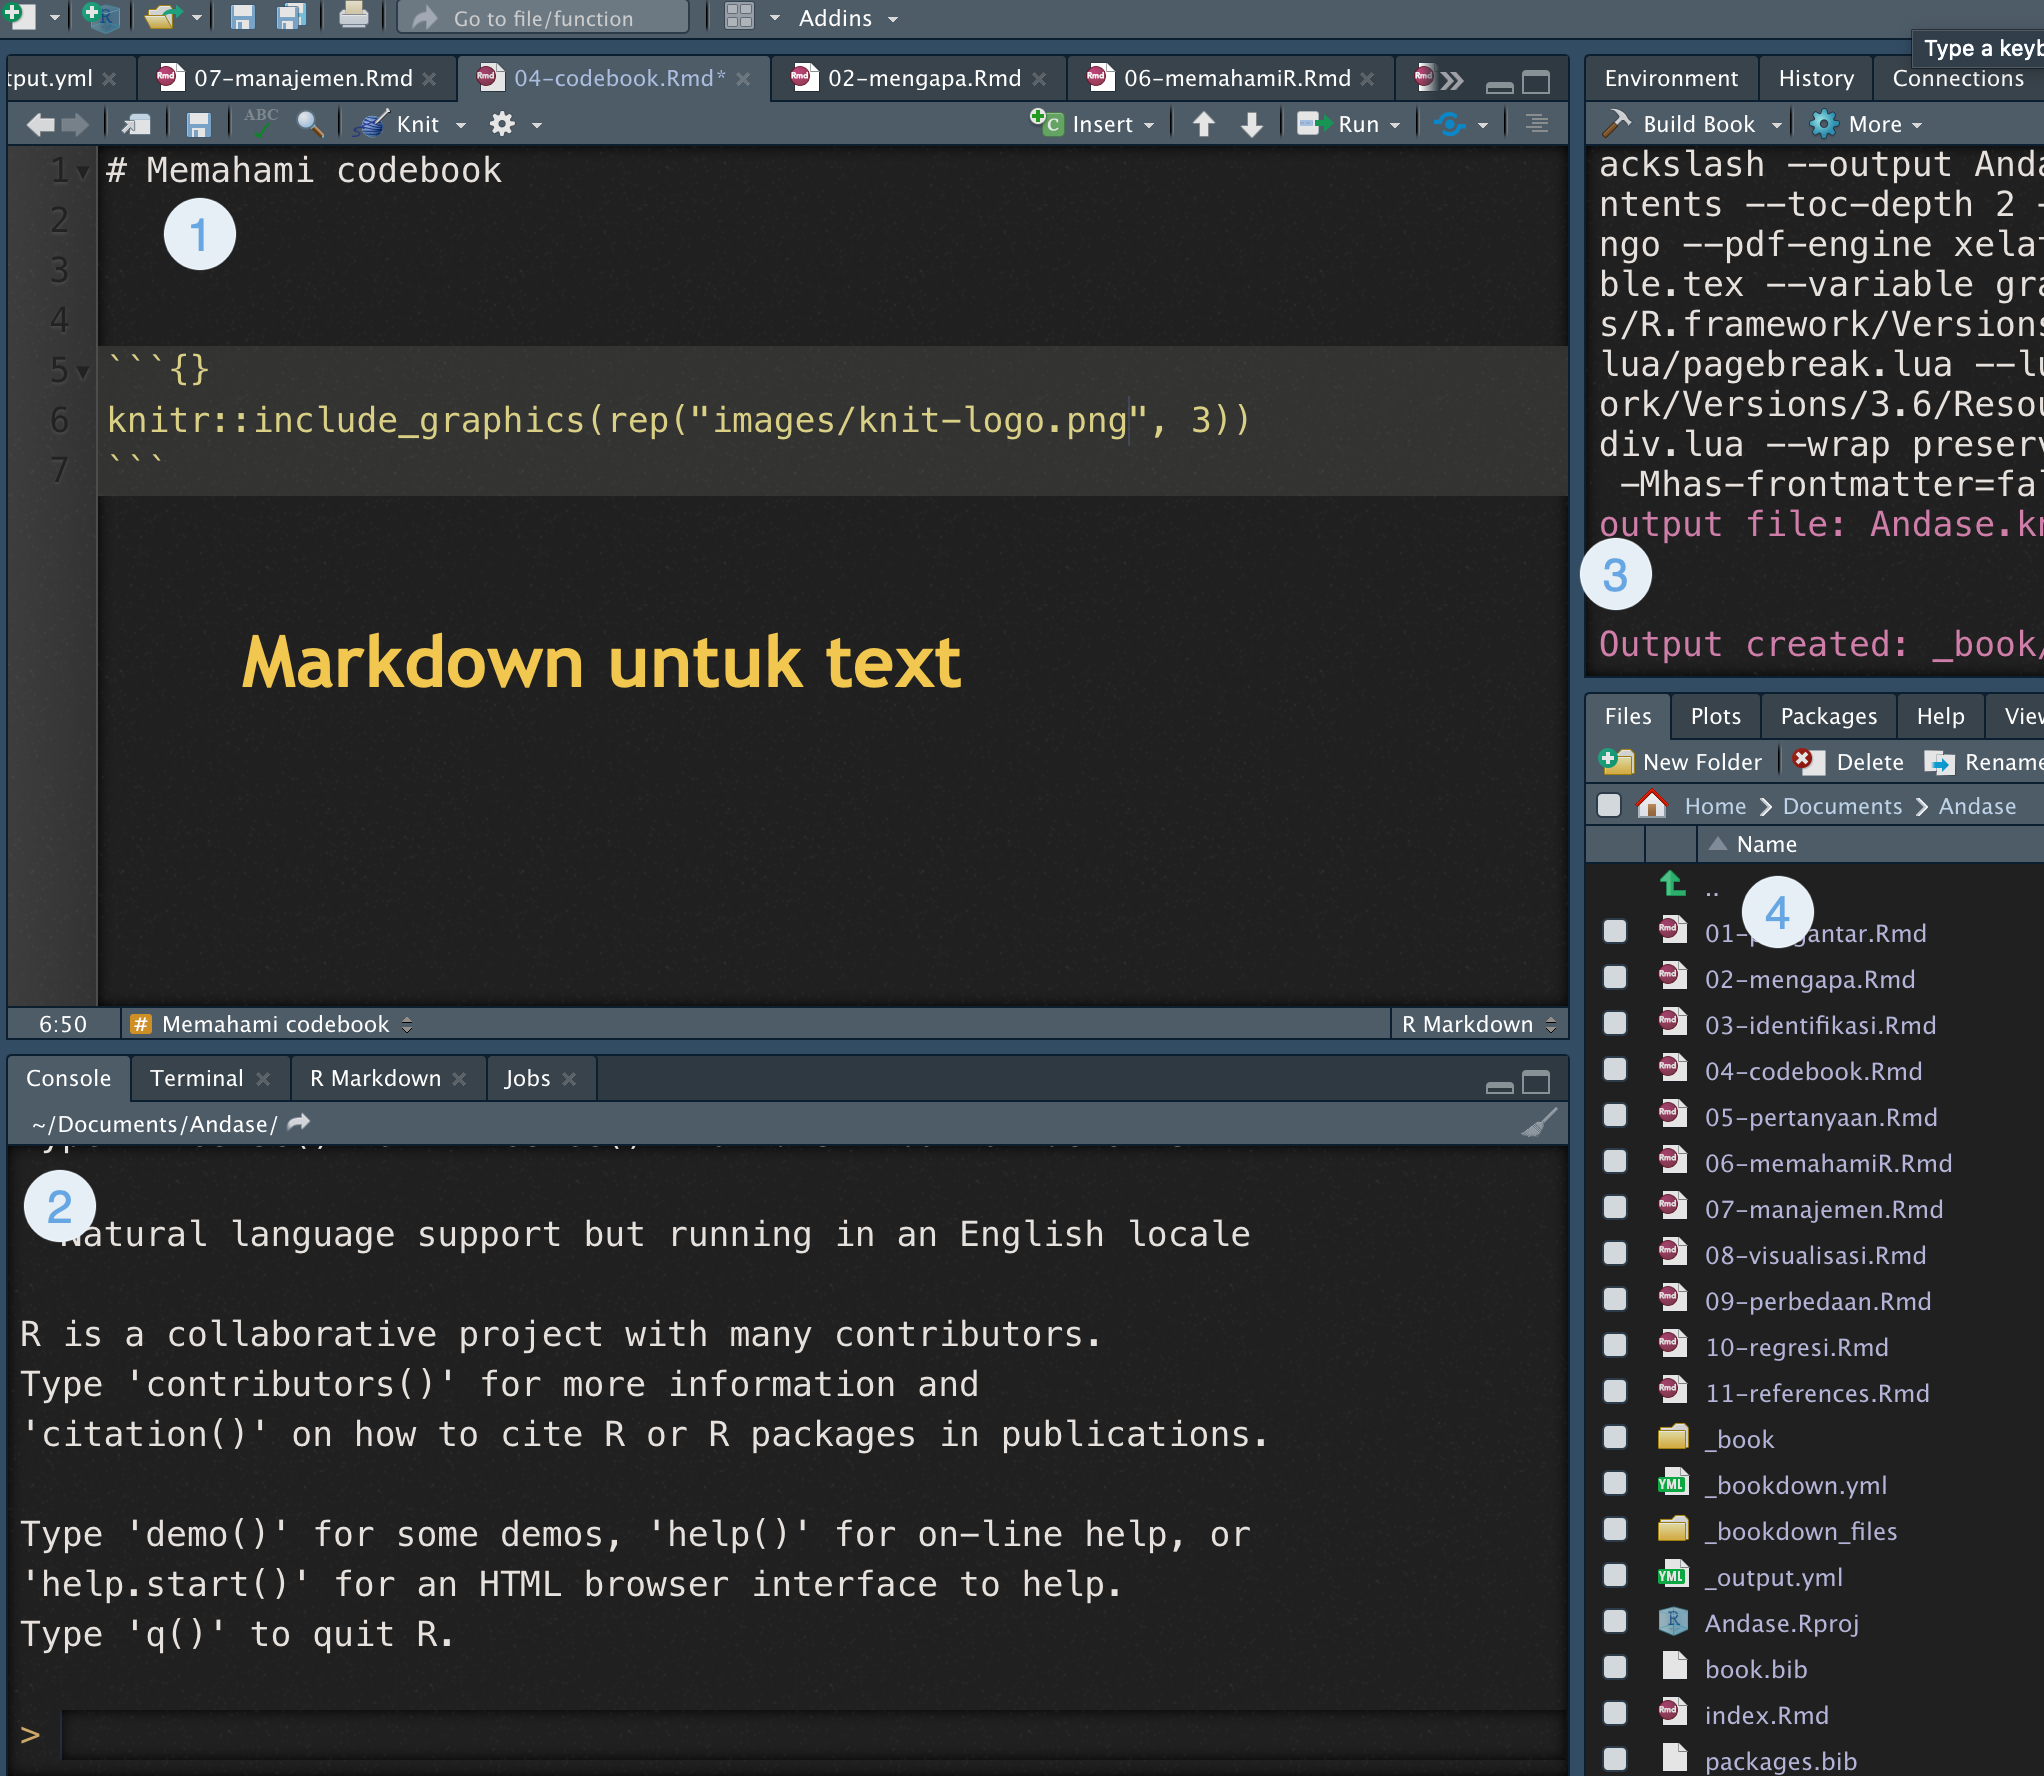
\includegraphics{rmda}
\end{verbatim}

\hypertarget{manajemen-data-1}{%
\chapter{Manajemen Data}\label{manajemen-data-1}}

\hypertarget{menggunakan-r}{%
\section{Menggunakan R}\label{menggunakan-r}}

\hypertarget{tidy-r}{%
\section{tidy R}\label{tidy-r}}

\hypertarget{filter}{%
\subsection{filter}\label{filter}}

\hypertarget{select}{%
\subsection{select}\label{select}}

\hypertarget{visualisasi-data}{%
\chapter{Visualisasi Data}\label{visualisasi-data}}

Visualisasi merupakan salah satu hal yang paling menarik dalam analisis data sekunder karena dapat memberi informasi yang padat namun mewakili apa yang ingin disampaikan penneliti. Salah satu rekomendasi paling baik untuk visualisasi data adalah R dengan paket ggplot2 dan lattice. ggplot2 merupakan implementasasi dari grammar of graphics dan emmungkinkan peneliti utnuk melakukan visualisasi data dengan pentahapan satu layer demi layer hingga menghasilkan visualisasi data yang elegan.

Salah satu paket yang paling banyak digunakan untuk visualisasi data dengan R adalah ggplot2 yang dibuat oleh Hadley Wickham. Pembahasan dan contoh mengenai paket ini dapat ditemukan dalam laman berikut ini: \url{http://docs.ggplot2.org/current/}. Laman ini memuat bagaimana sebuah visualisasi dihasilkan melalui kode R.

\#\#\#Pendahuluan

Memahami data merupakan salah satu kemampuan yang dibutuhkan untuk memahami statistika secara keseluruhan. Salah satu keunggulan yang dimiliki R adalah kemampuan untuk membuat grafik dan visualisasi data. R menyediakan visualisasi data dengan tingkat resolusi yang tinggi. Bab ini akan memberi penjelasan mengenai bentuk visualisasi data yang perlu digunakan dalam penelitian sosial. Selain itu, bab ini memberi contoh dan kode bagaiaman membuat plot data yang sedang diuji untuk memberi gambaran yang lebih menyeluruh mengenai data yang sedang diperiksa.

Bab ini membahas dan menjelaskan berbagai macam plot atau visualisasi data yang diperlukan dalam statistika, mulai dari bar plot, histogram, kernel density, box plot, violin plot, pie chart, scatter plot dan pembuatan peta. Pada masing-masing bentuk plot, akan dijelaskan pengertian plot, fungsi plot dan bagaimana mengimplementasikannya menggunakan R, serta penjelasan mengenai hasil plot yang diperoleh.

Dalam pemrograman R, ada beberapa package yang diperlukan untuk melakukan plot data dan visualisasi data dengan elegan adalah ggplot2, yang bisa digunakan dengan menuliskan kode berikut ini.

\begin{Shaded}
\begin{Highlighting}[]
\KeywordTok{library}\NormalTok{(gapminder)}
\KeywordTok{library}\NormalTok{(ggplot2)}
\NormalTok{gapminder}
\end{Highlighting}
\end{Shaded}

\begin{verbatim}
## # A tibble: 1,704 x 6
##    country     continent  year lifeExp      pop gdpPercap
##    <fct>       <fct>     <int>   <dbl>    <int>     <dbl>
##  1 Afghanistan Asia       1952    28.8  8425333      779.
##  2 Afghanistan Asia       1957    30.3  9240934      821.
##  3 Afghanistan Asia       1962    32.0 10267083      853.
##  4 Afghanistan Asia       1967    34.0 11537966      836.
##  5 Afghanistan Asia       1972    36.1 13079460      740.
##  6 Afghanistan Asia       1977    38.4 14880372      786.
##  7 Afghanistan Asia       1982    39.9 12881816      978.
##  8 Afghanistan Asia       1987    40.8 13867957      852.
##  9 Afghanistan Asia       1992    41.7 16317921      649.
## 10 Afghanistan Asia       1997    41.8 22227415      635.
## # … with 1,694 more rows
\end{verbatim}

Katakanlah kita ingin merencanakan Harapan Hidup terhadap PDB per kapita untuk semua tahun negara dalam data. Kami akan melakukan ini dengan membuat objek yang memiliki beberapa informasi yang diperlukan di dalamnya, dan membangunnya dari sana. Pertama, kita harus memberi tahu ggplot()fungsi apa data yang kita gunakan.

\begin{Shaded}
\begin{Highlighting}[]
\NormalTok{p \textless{}{-}}\StringTok{ }\KeywordTok{ggplot}\NormalTok{(}\DataTypeTok{data =}\NormalTok{ gapminder)}
\end{Highlighting}
\end{Shaded}

Pada titik ini ggplot tahu data kami, tetapi tidak tahu apa pemetaannya . Artinya, Anda tidak perlu secara eksplisit menyebutkan argumen yang Anda berikan ke fungsi, selama Anda memberikannya dalam urutan yang diharapkan, yaitu, urutan yang tercantum di halaman bantuan untuk fungsi tersebut.Kode ini akan tetap berfungsi jika kami menghapusdan.Dalam buku ini, saya menyebutkan semua argumen untuk kejelasan.kita perlu memberi tahu variabel mana dalam data yang harus diwakili oleh elemen visual mana dalam plot. Kami juga tidak tahu plot seperti apa yang kami inginkan. Di ggplot, pemetaan ditentukan menggunakan fungsi. Seperti ini:data = mapping =aes()

\begin{Shaded}
\begin{Highlighting}[]
\NormalTok{p \textless{}{-}}\StringTok{ }\KeywordTok{ggplot}\NormalTok{(}\DataTypeTok{data =}\NormalTok{ gapminder,}
            \DataTypeTok{mapping =} \KeywordTok{aes}\NormalTok{(}\DataTypeTok{x =}\NormalTok{ gdpPercap,}
                          \DataTypeTok{y =}\NormalTok{ lifeExp))}
\end{Highlighting}
\end{Shaded}

\begin{Shaded}
\begin{Highlighting}[]
\NormalTok{p }\OperatorTok{+}\StringTok{ }\KeywordTok{geom\_point}\NormalTok{()}
\end{Highlighting}
\end{Shaded}

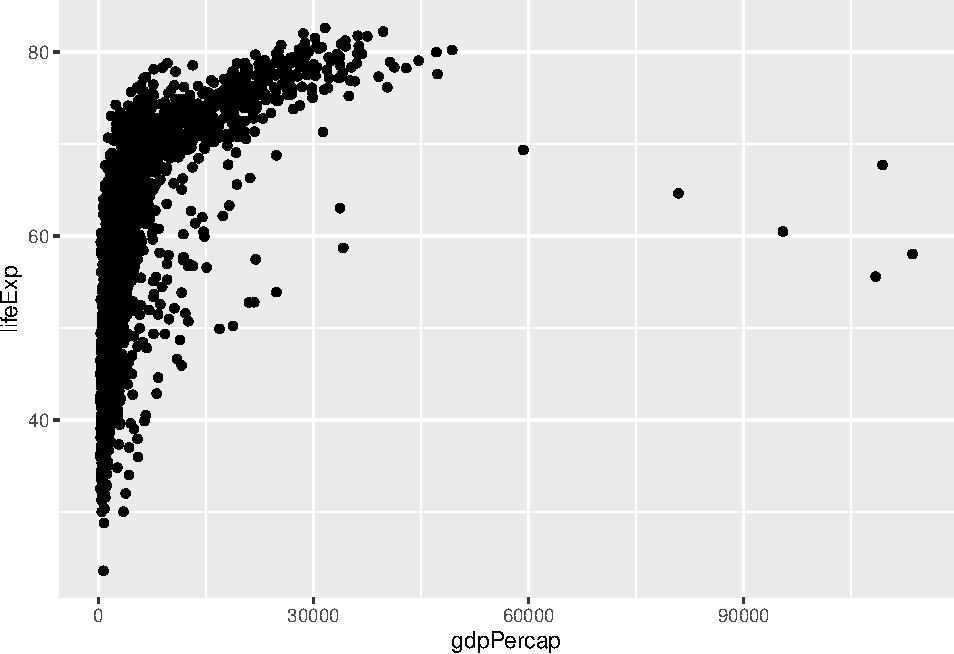
\includegraphics{Andase_files/figure-latex/unnamed-chunk-6-1.pdf}

\hypertarget{uji-perbedaan}{%
\chapter{Uji Perbedaan}\label{uji-perbedaan}}

\hypertarget{korelasi-dan-regresi}{%
\chapter{Korelasi dan Regresi}\label{korelasi-dan-regresi}}

  \bibliography{book.bib,packages.bib}

\end{document}
